\chapter{開発プロセス}

\section{ヒアリング}
 我々は町会の置かれている現状を明らかにするため、5月12日に町会に対してヒアリングを行った。町会役員から1.2で述べたイベント開催に関する問題と以下の要望が明らかになった。
\begin{itemize}
\item 開催予定のイベント一覧をカレンダーで表示して欲しい
\item iOSのアプリケーションを作って欲しい。
\item 幅広い年代の人が使いやすいUIにして欲しい。
\item 町会の役員の数を増やすため、町内会を知ってもらいたい。
\item イベント発信をした際に通知できる機能が欲しい。
\item イベントスケジュールでイベントの削除、作成、更新ができるようにして欲しい。
\item 行事をタップしたらそのまま参加申し込みフォームに遷移して欲しい。
\item 保護者の方の確認を得るためのポップアップ機能が欲しい。
\item イベントで不参加になった人が分かるようにして欲しい。
\end{itemize}
我々は、これらの要望の一部を取り入れつつ問題を解決するアプリケーションを開発することとした。
\section{アプリアイデアの考案}
1.2で述べた問題と町会の要望を分析した結果、イベントに関する内容のものが多かった。そこでイベントに関係する3つの問題を解決することとした。3つの問題は「FacebookやLINE@ではイベントに関するお知らせはできるが、開催予定のイベントを一覧で見れない」「Facebookでは個人情報が漏れてしまうため参加申し込みができない」「役員だけで共有したい情報を町民に知られずに共有することがFacebookやLINE@ではできない」である。これらの問題を解決するために、開催予定のイベントをカレンダー表示で見ることのできる機能、イベントの参加申し込みができる機能、参加申し込み者の情報を役員のみ見ることのできる機能、役員会議などのイベント情報を役員のみ見ることのできる機能をアプリケーションの機能として考案した。
アプリケーションアイデアの一部であるイベントカレンダー画面(図4.1)、参加フォーム画面(図4.2)、イベント作成画面(図4.3)を以下に示す。
\newpage
\begin{figure}[h]
    \begin{tabular}{ccc}
      %---- 最初の図 ---------------------------
      \begin{minipage}[t]{0.33\hsize}
        \centering
        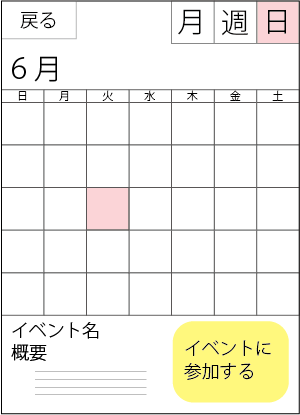
\includegraphics[keepaspectratio, scale=0.4]{process_figures/calender.png}
        \caption{イベントカレンダー画面}
        \label{calender}
      \end{minipage} &
      %---- 2番目の図 --------------------------
      \begin{minipage}[t]{0.33\hsize}
        \centering
        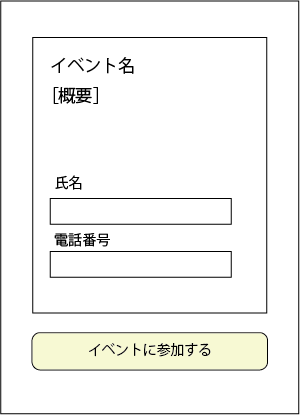
\includegraphics[keepaspectratio, scale=0.4]{process_figures/joinform.png}
        \caption{参加フォーム画面}
        \label{joinform}
      \end{minipage}
      %---- 3番目の図 --------------------------
      \begin{minipage}[t]{0.33\hsize}
        \centering
        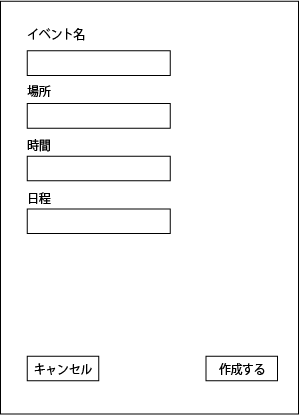
\includegraphics[keepaspectratio, scale=0.4]{process_figures/old_create_event.png}
        \caption{イベント作成画面}
        \label{create_event.old}
      \end{minipage}
      %---- 図はここまで ----------------------
    \end{tabular}
\end{figure}
\section{第1回提案・レビュー}
 5月30日に我々が考えたアプリケーションの画面イメージを町会に提案した。その結果、iOS、Android、Webアプリ3つに対応可能なアプリケーション開発を行うことが決定した。また、我々の考案したアプリケーションイメージについて、レビューで3つの要望を得た。1つ目は、イベント参加者の名簿を市役所に提出する際に参加者の情報として「名前」「性別」「年齢」「住所」「電話番号」が必要であるので、図1.bの入力フォームに5つの情報を追加して欲しいという要望である。2つ目は、アプリケーションをインストールした人が、すぐイベントを確認できるように起動時の画面はログイン画面にしないで欲しいという要望である。3つ目は、図1.bに「定員」の項目を追加して欲しいという要望である。提案時した資料については付録Aを参照されたい。
\section{アプリアイデアの改善}
4.3のレビューの内容を利用してアプリケーションアイデアを改善した。この改善に対して、教員より役員と町民でイベントカレンダーを共有することで本当に問題を解決できるのかと指摘を受け、アプリケーションについて再考し改善を図った。その結果、カレンダーを用いて開催予定のイベントを表示するのではなく、開催予定のイベントを直近のものから順にリスト表示することにした。理由として、カレンダー表示では来月の予定などがひと目で確認することができないからである。
アプリケーションアイデアの一部であるイベントリスト画面(図4.4)、イベント作成画面(図4.5)、参加者リスト画面(図4.6)を以下に示す。
\newpage%苦肉の策
\begin{figure}[h]
    \begin{tabular}{ccc}
      %---- 最初の図 ---------------------------
      \begin{minipage}[t]{0.3\hsize}
        \centering
        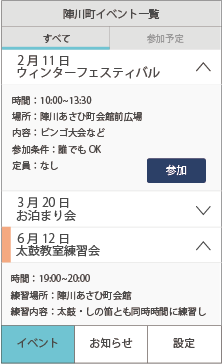
\includegraphics[keepaspectratio, scale=0.5]{process_figures/eventlist.png}
        \caption{イベントリスト画面}
        \label{calender}
      \end{minipage} &
      %---- 2番目の図 --------------------------
      \begin{minipage}[t]{0.3\hsize}
        \centering
        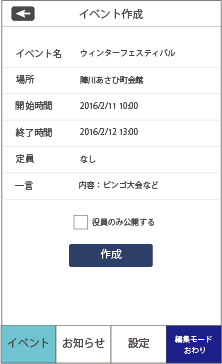
\includegraphics[keepaspectratio, scale=0.5]{process_figures/new_create_event.png}
        \caption{イベント作成画面}
        \label{joinform}
      \end{minipage}
      %---- 3番目の図 --------------------------
      \begin{minipage}[t]{0.3\hsize}
        \centering
        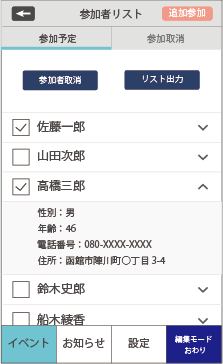
\includegraphics[keepaspectratio, scale=0.5]{process_figures/joinlist.png}
        \caption{参加者リスト画面}
        \label{create_event.old}
      \end{minipage}
      %---- 図はここまで ----------------------
    \end{tabular}
\end{figure}
\section{第2回提案・レビュー}
 6月23日に我々は町会に対して改善したアプリケーションイメージを提案した。その結果、画面ごとにレビューしてもらい詳細な要望を受けた。具体的には、図2.aでイベントをタップすると画面いっぱいにイベントの詳細情報が表示されるようにして欲しいという要望、図2.bでにアプリケーションの所有者全員に通知するかしないかの項目を設けて欲しいという要望である。また、町民が利用したくなるようなコンテンツを追加して欲しいという要望も得た。過去のイベントの写真が確認できるWebページとアプリケーションとリンクさせることが例として挙げられる。提案した資料については付録Bを参照されたい。
\bunseki{永井陽太}
